\subsection*{Overview}

We turned scanned USGS reports into machine-readable tables, each with metadata giving its location, dates and content, in three automated steps: table detection, digitization and metadata extraction (Fig. M1; one example table followed through all three steps in Fig. M2). Each step was evaluated against hand-checked pages.

Reports were found by searching the USGS Publications Warehouse for California reports published 1879--1980 that matched water-related keywords (wells, groundwater, stream, discharge, springs, irrigation and 21 other terms) (Supplementary Note 1). The search returned 1,042 reports. Of these, 629 (60\%) were available as scanned PDFs, 104,729 pages in all. Every page was rendered at 300 dpi and saved as a grayscale PNG (pdf2image).

\begin{figure}[htbp]
\centering
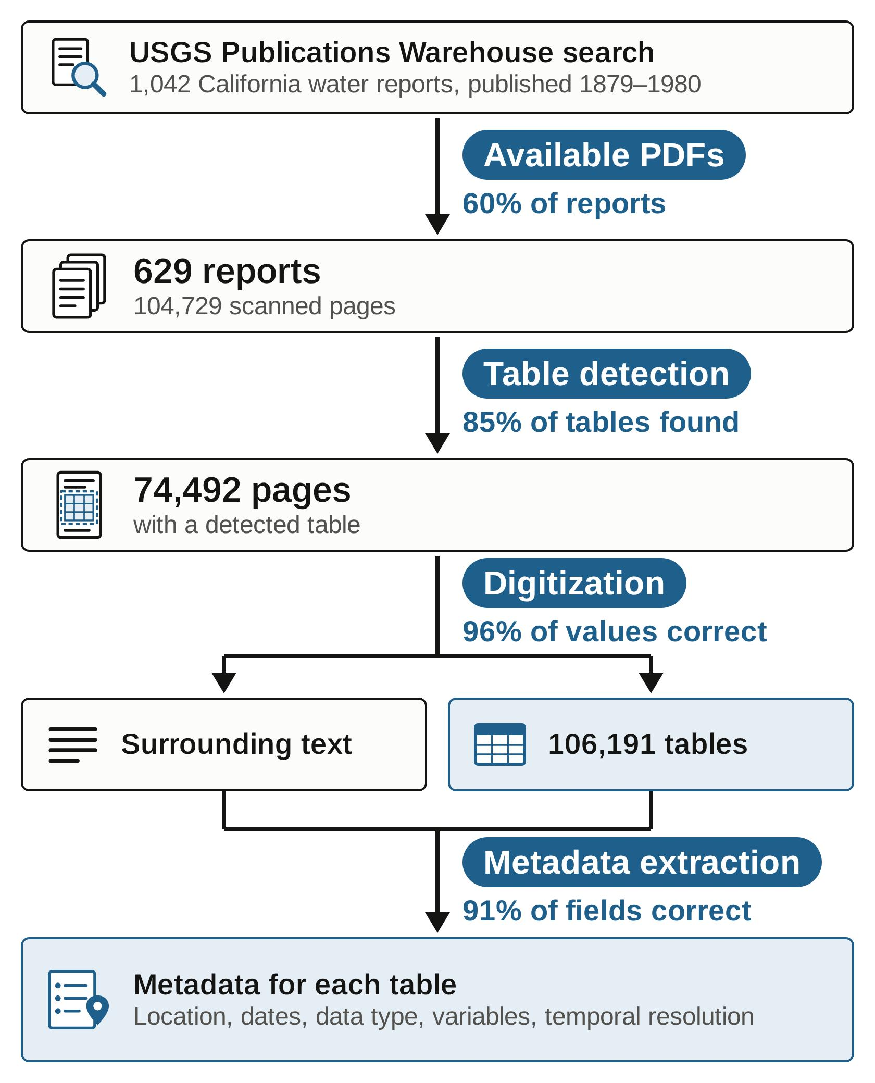
\includegraphics[width=0.6\textwidth]{../figures/methods_overview.pdf}
\caption*{\textbf{Figure M1.} The digitization pipeline. Black boxes are inputs and intermediate products, blue boxes are the published products, and blue labels are the steps. Under each automated step is its measured accuracy: the share of known table pages the detector found at the stricter of its two thresholds (0.8), the share of printed numbers Reducto read correctly and placed under the right row and column, and the share of metadata fields right, averaged over eight fields. Surrounding text is the page text Reducto returns along with the tables.}
\label{fig:methods-overview}
\end{figure}

\begin{figure}[htbp]
\centering
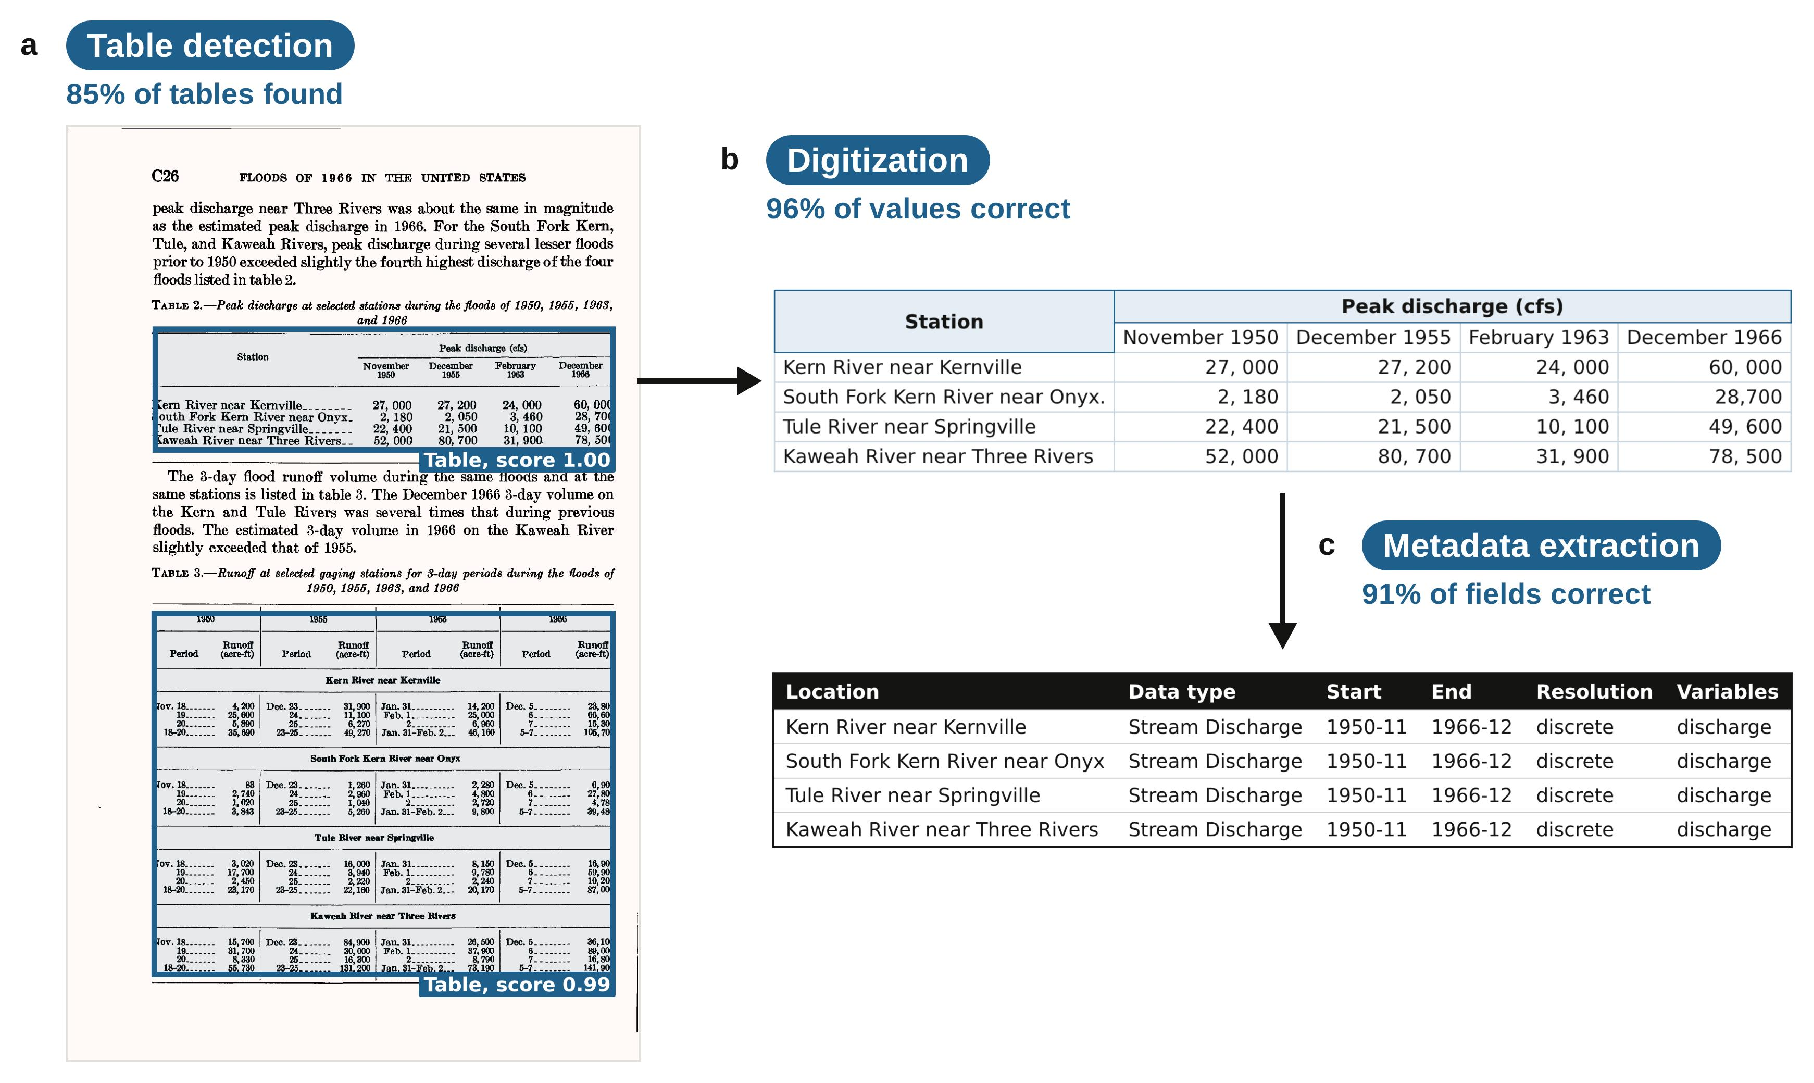
\includegraphics[width=\textwidth]{../figures/methods_example.pdf}
\caption*{\textbf{Figure M2.} One table followed through the pipeline, from printed page C26 of Floods of 1966 in the United States. (a, left) The scanned page with the detector's boxes and confidence scores. (b, top right) Reducto's output for the first table, unedited. (c, bottom right) The metadata returned for that table, one row per location; six fields are shown. Accuracies are those of Figure M1.}
\label{fig:methods-example}
\end{figure}

\subsection*{Table detection}

Because not every page in the reports contained usable tabular data and digitizing every page would be prohibitively expensive, we first used Table Transformer to locate where in the reports there were tables to be digitized (Smock et al. 2022). The detector found 85\% of known tables at the stricter of the two thresholds used (0.8), and about 11\% of the pages it flagged held no table (Table M1). This process led to 74,492 of the 104,729 pages (71\%) being flagged for digitization.

\textbf{Approach.} Each page image was binarized (Otsu), resized so its longer side was 800 pixels, and passed to Table Transformer (Smock et al. 2022), which returns boxes labeled table or rotated table with a confidence score (Figure M2a). A page was sent on to digitization if any box scored at or above the threshold. The threshold was 0.75 for the 270 reports published 1971--1980 (43\% of reports, 34\% of pages) and 0.8 for the 359 reports published 1898--1970 (57\% of reports, 66\% of pages). In total, 74,492 pages were flagged.

\textbf{Evaluation.} While a false positive leads us to digitize a page without a table, leading to inefficiencies in the pipeline, a false negative leads to losses in the amount of data digitized. Therefore, our main evaluation metric is recall, or the number of pages with tables that were identified.

Recall was measured against an existing hand-compiled list of report pages that hold groundwater tables (139 USGS reports, mostly outside California, CITE Annette's paper). To clean the list of pages with no table, we manually checked every listed page. Listed pages with no table were removed (73 pages), and 27 listed pages that pointed to the page beside a table were moved to it, leaving 3,272 pages. Recall is the share of these pages with a box at or above the threshold. Its 95\% interval comes from resampling reports (2,000 resamples).

In order to capture the inefficiency of the pipeline, we also calculate the false-alarm rate: the share of flagged pages with no table. We first took the share of flagged pages for which Reducto returned no table (9.7\% at 0.75). We then corrected it by looking at 60 of those pages and 300 pages for which Reducto did return a table. Reducto was wrong in both directions: 3 of the 60 pages held a table it had missed (57 had none), and 9 of the 300 held no table. Weighting each sample's no-table rate by its group's share of flagged pages gives the corrected rate.

\begin{table}[htbp]
\centering
\small

\caption*{\textbf{Table M1.} Table detection at the two thresholds used. Recall is the share of the 3,272 listed pages with a table that have a detector box scoring at or above the threshold. False alarms are the share of flagged pages with no table. Values in brackets are 95\% intervals, from 2,000 resamples of reports for recall and from resamples of the hand-labelled pages within each group for false alarms.}
\begin{tabularx}{\textwidth}{>{\raggedright\arraybackslash\hspace{0pt}}X>{\raggedright\arraybackslash\hspace{0pt}}X>{\raggedright\arraybackslash\hspace{0pt}}X>{\raggedright\arraybackslash\hspace{0pt}}X}
\toprule
\textbf{Threshold} & \textbf{Recall} & \textbf{Tables found} & \textbf{False alarms among flagged pages} \\
\midrule
0.75 & 87.5\% (84.0--90.7) & 2,863 of 3,272 & 11.9\% (10.3--13.9) \\
0.8 & 85.3\% (81.5--88.5) & 2,791 of 3,272 & 11.0\% (9.3--13.0) \\
\bottomrule
\end{tabularx}
\end{table}

\subsection*{Digitization}

Once the tables to be digitized were located, we used Reducto to digitize the information within each table. Reducto read 96\% of printed numbers correctly and placed them under the right row and column (Table M2). The open-source model PaddleOCR, which we tested first, only achieved 1\%.

\textbf{Approach.} Each flagged page was sent to Reducto (reducto.ai, commercial API, 2024), which returns the page as text blocks and tables (HTML) with bounding boxes. We kept the full output as JSON, though we also converted each table to a CSV file to improve accessibility. PaddleOCR (open source) was tested on the same pages and rejected.

\textbf{Evaluation.} We transcribed tables from 20 pages at random from 57 reports: 4 pages for each kind of table (daily, monthly, annual, discrete measurements, no time series), at most one page per report. The tables were transcribed from the page images by Claude Fable 5.2 (Anthropic) without access to either tool's output, then read against the scans by one author, who found no errors beyond the typing of superscripts and subscripts, which was corrected. The 20 pages hold 32 tables and 4,696 printed numbers.

A model is evaluated by scoring the percent of printed numbers that are both correct and sorted under a correct row label and column header, so that a user could find it. Rows and columns of the output were matched to the printed table in order, maximizing agreement (Supplementary Note 2). Labels were compared ignoring case, spacing, punctuation, leader dots and line-break hyphens. Number formatting was compared leniently: printed gaps (``21. 2'', ``4, 400'') were closed and a lone letter o was read as zero (under strict formatting Reducto scores 91.1\%). Because the test pages were drawn in equal numbers for each kind of table, the counts for each kind were scaled by the number of pages of that kind in the corpus (daily 66\%, discrete 15\%, monthly 12\%, annual 5\%, no time series 3\%), so that the results estimate the share of all numbers in the corpus. Performance by table type is reported in Supplementary Table 1. The 95\% ranges come from 5,000 resamples of pages within kinds.

\begin{table}[htbp]
\centering
\small

\caption*{\textbf{Table M2.} Digitization accuracy by tool and output format: Reducto (raw HTML and converted to CSV) and PaddleOCR. Percentages are shares of printed numbers, with every number counting equally and each kind of table scaled by its number of pages in the corpus; each column adds to 100\% up to rounding. Values in brackets are 95\% ranges from 5,000 resamples of pages within kinds.}
\begin{tabularx}{\textwidth}{>{\raggedright\arraybackslash\hspace{0pt}}X>{\raggedright\arraybackslash\hspace{0pt}}X>{\raggedright\arraybackslash\hspace{0pt}}X>{\raggedright\arraybackslash\hspace{0pt}}X}
\toprule
\textbf{Outcome} & \textbf{Reducto, raw output (HTML)} & \textbf{Reducto, converted to CSV} & \textbf{PaddleOCR} \\
\midrule
Right number under the right row and column & 96.1\% (93.5--98.3) & 86.9\% (80.7--92.9) & 1.2\% (0.4--2.3) \\
Right number, wrong row label & 0.0\% & 0.0\% & 1.7\% \\
Right number, wrong column header & 1.0\% & 10.2\% & 1.9\% \\
Right number, both labels wrong & 0.0\% & 0.0\% & 8.5\% \\
Wrong number & 1.7\% & 1.7\% & 22.5\% \\
Cell missing from a table that was found & 0.2\% & 0.2\% & 48.7\% \\
Whole table missed & 1.0\% & 1.0\% & 15.6\% \\
Tables found (of 32) & 29 (1 split, 2 missed) & 29 (1 split, 2 missed) & 22 (10 missed) \\
\bottomrule
\end{tabularx}
\end{table}

The CSV conversion loses accuracy because multi-level column headers are flattened (10.2\% of numbers end up under the wrong column header, against 1.0\% in the raw output); the numbers themselves are unchanged. The two tables Reducto missed are rotated tables, returned as a transposed, scrambled grid.

\subsection*{Metadata extraction}

In order for the digitized tables to be discoverable and therefore useful to researchers, it is important to know what they contain, or metadata. We therefore deigned a pipeline to extract location, date, and content information for each table. On a held-out test set of 200 tables, the pipeline got 91\% of metadata fields right on average (Table M3).

\textbf{Approach.} In addition to the digitized tables, Reducto returned all text of each page fully digitized. Each page was processed on its own by an open-weight language model, Qwen3.6-27B (FP8 weights, Apache-2.0 license) with reasoning turned off. The input was Reducto's text for the page with its tables numbered in reading order. For each numbered table the model returned every location the table covers and, for each location, the evidence printed on the page, copied verbatim: coordinates, well number, station number or name, township-range-section, place name with its relation (at, near, below), basin or area, county and state. It also returned the water source, data type (one of nine categories: stream discharge, groundwater, reservoir, irrigation, springs, precipitation, water quality, not water related, other), start and end dates (as precise as printed: 1916, 1916-10 or 1916-10-01), temporal resolution (daily, monthly, annual, discrete, no time series), the variables recorded (from a fixed list) and, for wells, the date of construction. The full prompt is found under Supplementary Note 3, in addition to three data cleaning steps that follow the prompt. Each location was then given the most specific evidence available, in the order coordinates, well number, station number, station name, township-range-section, place name, basin or area, county, state. The output has one row per location per table. The pipeline was run on all 106,319 digitized tables and extracted metadata for all but 152 (0.1\%), where the model's answer was unreadable (72 tables) or left the table out (62), or Reducto had kept no page text (18). For these 152 tables, Claude Fable 5.2 (Anthropic) read the page scan and recorded the same fields following the answer-key rules (Supplementary Note 4).

\textbf{Evaluation.} The test set is 200 tables from 137 reports, drawn at random within four groups of data type (80 stream discharge, 50 groundwater, 35 reservoir, 35 other types), one table per page and at most three per report. Pages used during development and pages on tribal lands were excluded. The prompt and rules were developed on two separate validation sets of 100 tables each; the test set was scored once, after the pipeline was frozen.

The answer key was written from the page images by Claude Fable 5.2 (Anthropic), blind to the pipeline's output, following written rules (Supplementary Note 4). One author checked the first 20 tables and found no errors; the rest of the key was not checked by hand. A field is counted right if the page gives a value and the output matches it. Dates match if they agree to the precision of the key, variables if the sets are equal, and coordinates if their digits agree. Results are weighted to the published tables by the share of each data-type group.

\begin{table}[htbp]
\centering
\small

\caption*{\textbf{Table M3.} Metadata fields and their accuracy on the test set (200 tables, 289 rows, one per location per table). Accuracy is the share of rows for which the page gives the field and the output matches it. Tables are weighted by how common their data type is among the published tables (stream discharge 84\%, groundwater 8\%, reservoir 4\%, other types 4\%). Values in brackets are 95\% ranges from 5,000 resamples of tables within data-type groups. Examples are the first row of the table in Figure M2.}
\begin{tabularx}{\textwidth}{l>{\raggedright\arraybackslash}Xll}
\toprule
\textbf{Field} & \textbf{What it records} & \textbf{Example} & \textbf{Accuracy (95\% range)} \\
\midrule
Location & The most specific location evidence printed on the page for the site & Kern River near Kernville & 92\% (88--96) \\
Location type & The kind of evidence the location is: coordinates, well number, station number, station name, township-range-section, named place, basin or area, county or state & station name & 94\% (90--97) \\
Water source & Name of the river, creek, canal, lake, reservoir, spring or well & Kern River & 91\% (86--95) \\
Data type & The kind of water the site is on, one of nine categories & Stream discharge & 96\% (93--99) \\
Start date & First measurement in the table for the location, as precise as printed & 1950-11 & 83\% (76--90) \\
End date & Last measurement in the table for the location, as precise as printed & 1966-12 & 84\% (77--91) \\
Temporal resolution & Daily, monthly, annual, discrete or no time series & discrete & 95\% (91--98) \\
Variables & What the table records, from a fixed list of 17 & discharge & 92\% (88--96) \\
Mean of the eight fields &  &  & 91\% (88--93) \\
\bottomrule
\end{tabularx}
\end{table}

The number of locations per table was right for 98\% of tables, and the construction date for 81\% of the 19 rows that print one. The 91\% headline is the mean of the eight fields from location to variables. Judged by year alone, the start date was right for 87\% of rows (95\% range 81--93) and the end date for 96\% (92--99). Results for each group of data types are in Supplementary Table 2.
